\section{Results and interpretation}
\label{sect:stat}
The observed data and predicted background yields for the four signal regions are summarized in Table~\ref{tbl:yieldSysSummary}. 
\begin{table}[!htb]
\begin{center}
%\begin{tiny}
\caption{Data yields and background predictions with uncertainties in the four signal regions of the search. 
%The first two lines are based on Monte Carlo simulation, when for the first row, a validation against data is also done. 
%The last two rows are data driven, but the ``Fake'' for the \tauTau channel is not completely data driven.
%The uncertainties are systematic, unless when there are two parts, the first part is statistics.
The uncertainties are reported in two parts, the statistical and systematic uncertainties, respectively. 
%For \wjets in \tauTau channel, the full uncertainty is
%reported and considered as systematic for ``SM Total''.
The main backgrounds (\wjets and QCD multijet) are derived from data as described in Section~\ref{sect:bkg},
The abbreviation ``VV'' refers to diboson events.
}
\begin{tabular}{|c|c|c|c|c|}
\hline
	           & \eTau & \muTau & \tauTau \binone & \tauTau \bintwo \\
\hline
 Z+jets            & 0.19 $\pm$ 0.04 $\pm$ 0.03 & 0.25 $\pm$ 0.06  $\pm$ 0.04  &  0.56 $\pm$ 0.07 $\pm$ 0.12 & 0.81 $\pm$ 0.56 $\pm$ 0.18  \\
\ttbar, VV, hX  & 0.03 $\pm$ 0.03 $\pm$ 0.02 & 0.19 $\pm$ 0.09  $\pm$ 0.09  &  0.19 $\pm$ 0.03 $\pm$ 0.09 & 0.75 $\pm$ 0.35 $\pm$ 0.38  \\
\wjets             & 3.30 $\pm$ 3.35 $\pm$ 0.56 & 8.15 $\pm$ 4.59  $\pm$ 1.53  &  0.70 $\pm$ 0.21 $\pm$ 0.55 & 4.36 $\pm$ 1.05 $\pm$ 1.63  \\
QCD multijet       &             -              &            -                 &  0.13 $\pm$ 0.06 $\pm$ 0.21 & 1.15 $\pm$ 0.39 $\pm$ 0.74  \\
\hline
SM total           & 3.52 $\pm$ 3.35 $\pm$ 0.56 & 8.59 $\pm$ 4.59  $\pm$ 1.53  &  1.58 $\pm$ 0.23 $\pm$ 0.61 & 7.07 $\pm$ 1.30 $\pm$ 1.84  \\
\hline
\hline
Observed           &               3            &                5             &             1               & 2     \\  
\hline
\end{tabular}
\label{tbl:yieldSysSummary}
\end{center}
\end{table}

In all signal regions the observed data yields are consistent with the predicted SM background yields.

Figure \ref{fig:yield_final}
\begin{figure}[!Hhtb]
\centering
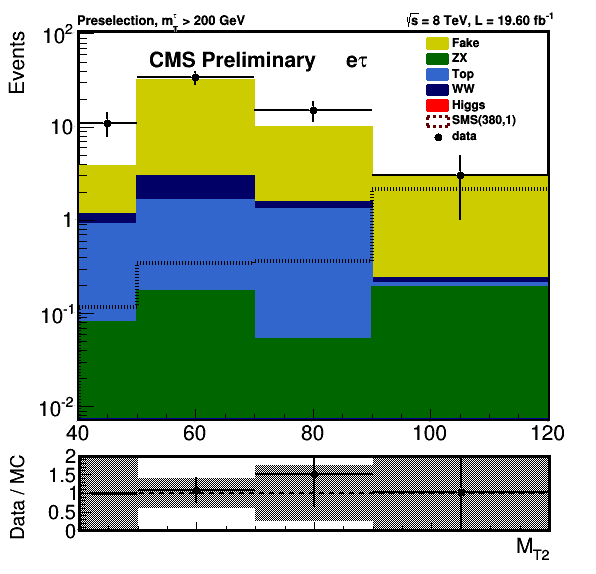
\includegraphics[width=0.475\textwidth,keepaspectratio=true]{StatisticsFig/MT2_tauMTgt200_DDFakeEleTau.png}
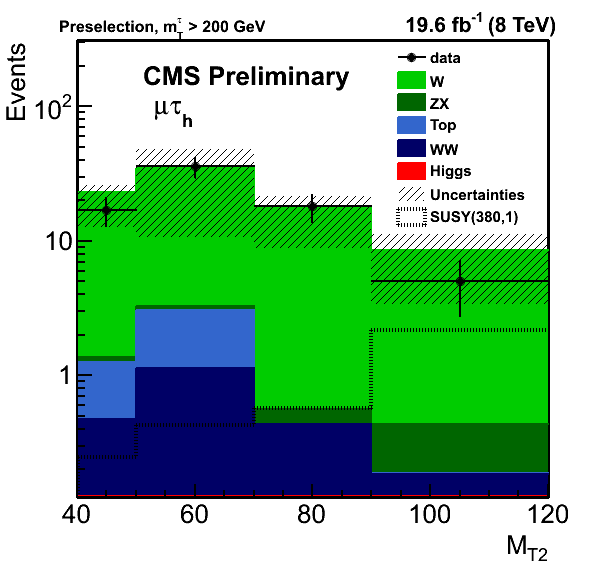
\includegraphics[width=0.475\textwidth,keepaspectratio=true]{StatisticsFig/MT2muTau_tauMTgt200_DDFake.png}
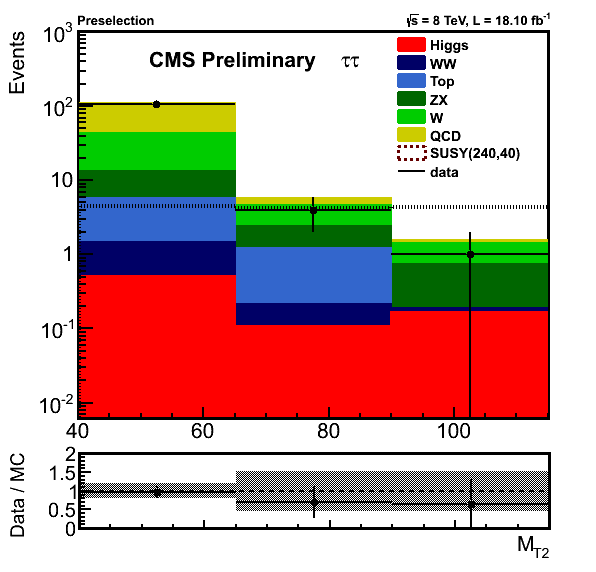
\includegraphics[width=0.475\textwidth,keepaspectratio=true]{StatisticsFig/QCDWestimation_bin1.png}
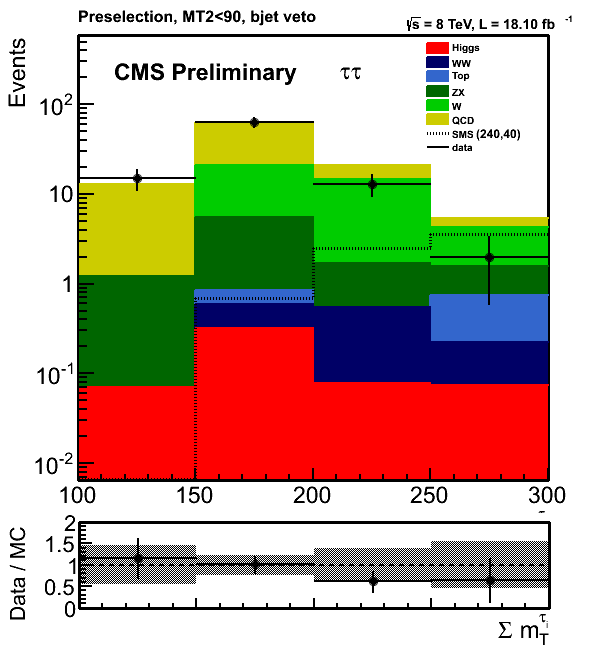
\includegraphics[width=0.475\textwidth,keepaspectratio=true]{StatisticsFig/QCDWestimation_bin2.png}
\caption{The data yield is compared with the Standard Model expectation. In different signal regions, 
when a data driven background is available, it is used instead of the pure simulation. For more details read the text.}
\label{fig:yield_final}
\end{figure}
compares the data and the Standard Model expectation in different channels. The top row 
shows the \mttwo distributions in the \leptonTau channels. 
In these plots, the QCD multijet and \wjets and fake contribution from other channels are shown 
as ``Fake'' which were described in Section \ref{sect:bkgFake}.
The bottom row shows the \mttwo and \SumMT distributions in two different signal regions of \tauTau channel. 
The QCD multijet contribution in these plots comes from the data driven method described in 
Section \ref{sect:bkgQCD}. The \wjets contribution in the last bin of the bottom plots was described in Section \ref{sect:bkgW}. 
The uncertainty band in these 4 plots, includes both the statistical and systematical uncertainties.

There is no excess of events over the SM expectation.  We interpret our results in the context
of a simplified model of chargino pair production and decay, which was described in Section~\ref{sect:MCSamples} and corresponds 
to the left diagram in Fig.~\ref{fig:Productions}. 

A modified frequentist approach, known as the CLs method \cite{read:CLs}, is used to 
set limits on cross sections at 95\% confidence level.
Combining all four signal regions,
the expected(observed) limits rule out \chione  masses up to 400(430)\GeV  for a massless \PSGczDo and  
\PSGczDo masses up to 90(120)\GeV for some  \chione masses,
see Fig.~\ref{fig:limit_final}. 
%%%%%%%%%%
\begin{linenomath}
\begin{figure}[!Hhtb]
\centering
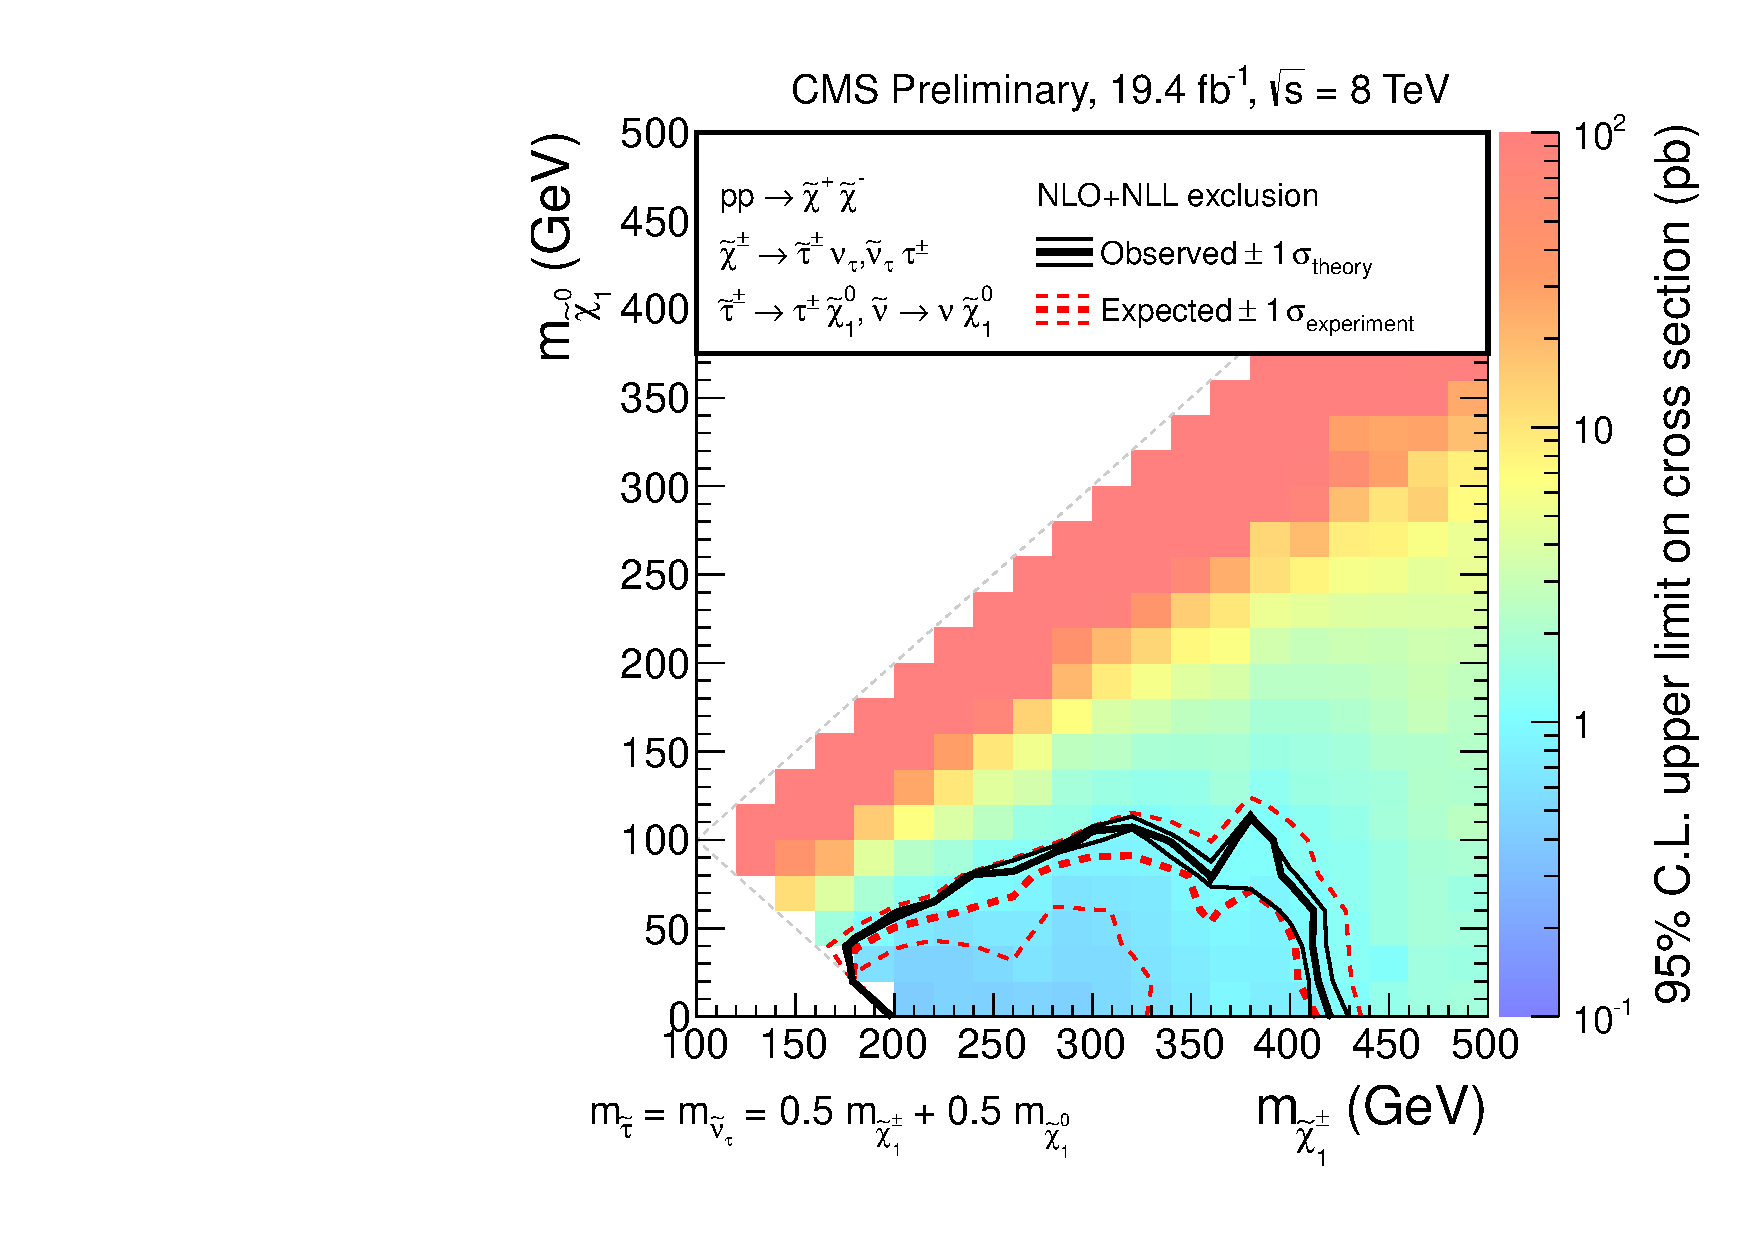
\includegraphics[width=0.7\textwidth,keepaspectratio=true]{StatisticsFig/Exclusion4Bins.pdf}
\caption{Expected and observed exclusion power in terms of Simplified Models
with the total dataset of 2012. The bottom-left triangle was excluded by LEP \sTau searches. 
The diagonal line denotes the boundary for $m_{\chione} = m_{\tau} + m_{LSP}$.
The one standard deviations of the expected (observed) exclusions introduced by the experimental 
(theoretical) uncertainties are also shown.}
\label{fig:limit_final}
\end{figure}
\end{linenomath}
%%%%%%%%%%
The boundaries are well beyond the ATLAS reach which is \chione  masses up to 345\GeV \cite{Aad:2014yka}. Adding \leptonTau channels
and considering two signal regions in \tauTau channel has increased the sensitivity of the current search compared to ATLAS which uses only 
one search region in \tauTau channel to make the exclusion.
The \sTau searches in the LEP experiments \cite{lepsusy} have excluded masses below 95\GeV. In Fig.~\ref{fig:limit_final}, 
this region corresponds to the triangle in bottom-left corner. % is shown by the line labeled as $m_{\sTau} < 95\GeV$. 
The diagonal line denotes the boundary for $m_{\chione} = m_{\tau} + m_{LSP}$, which is the kinematical boundary of the search.
The expected limits and their one standard deviations introduced by the experimental 
uncertainties are shown with the red solid and dashed lines, respectively. The observed limits are shown with the black solid lines, the one 
standard deviations are shown with narrower black lines. The theoretical cross sections are moved up and down by one one standard deviation to 
find the narrow lines.
The signal cross sections in NLO + next-to-leading-logarithm (NLL) order in $\alpha_s$ are used to make the exclusion limits.
In the whole region, the observed limits are within one standard deviation from the expected limits.  

The exclusion limits when only the \tauTau channels are used is shown in Fig.~\ref{fig:limit_tauTau}.
\begin{linenomath}
\begin{figure}[!Hhtb]
\centering
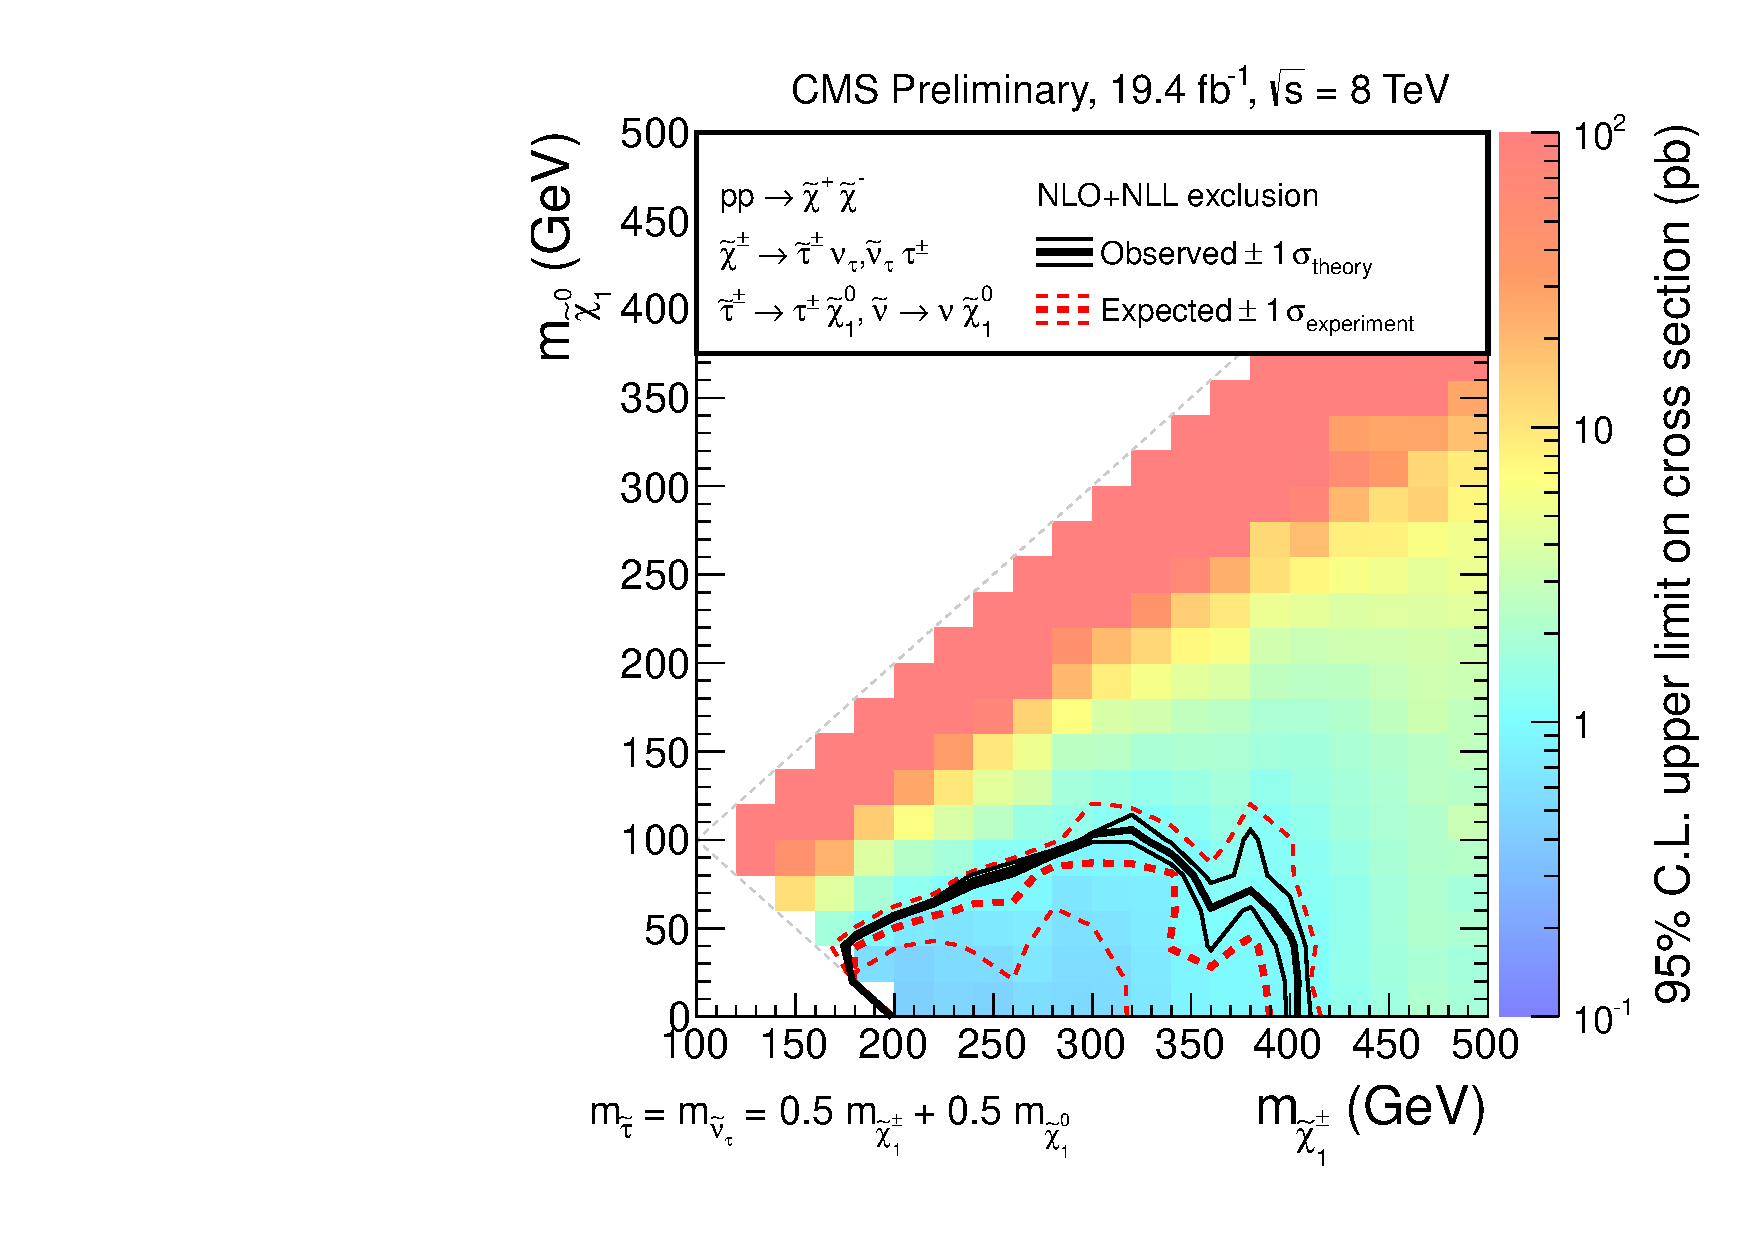
\includegraphics[width=0.7\textwidth,keepaspectratio=true]{StatisticsFig/ExclusionTauTau2Bin.pdf}
\caption{Expected and observed exclusion power in terms of Simplified Models
in combination of \tauTau channels. The conventions are same as Fig.~\ref{fig:limit_final}.}
\label{fig:limit_tauTau}
\end{figure}
\end{linenomath}
Even in this case, still the results are comparable with ATLAS results, 
due to the tighter signal selection and combining two sihnal regions statistically.


The results of the \tauTau channels are interpreted to set limit on the $\tilde{\tau}\tilde{\tau}$ production, 
which corresponds to the right diagram in Fig.~\ref{fig:Productions}. 
In this simplified model, two $\tilde{\tau}$ are directly produced from the $pp$ collision and decay instantly 
into two $\tau$ and two \PSGczDo. Two $\ell\Tau$ channels are not considered in this interpretation, because they do not improve the results. 
As the cross section of direct production of sleptons is lower, no point is excluded and a $95\%$ upper limit is set on 
the cross section  as a function of the stau mass. 
Figure \ref{fig:limit_stau_stau} represents the ratio of the 
\begin{linenomath}
\begin{figure}[!Hhtb]
\centering
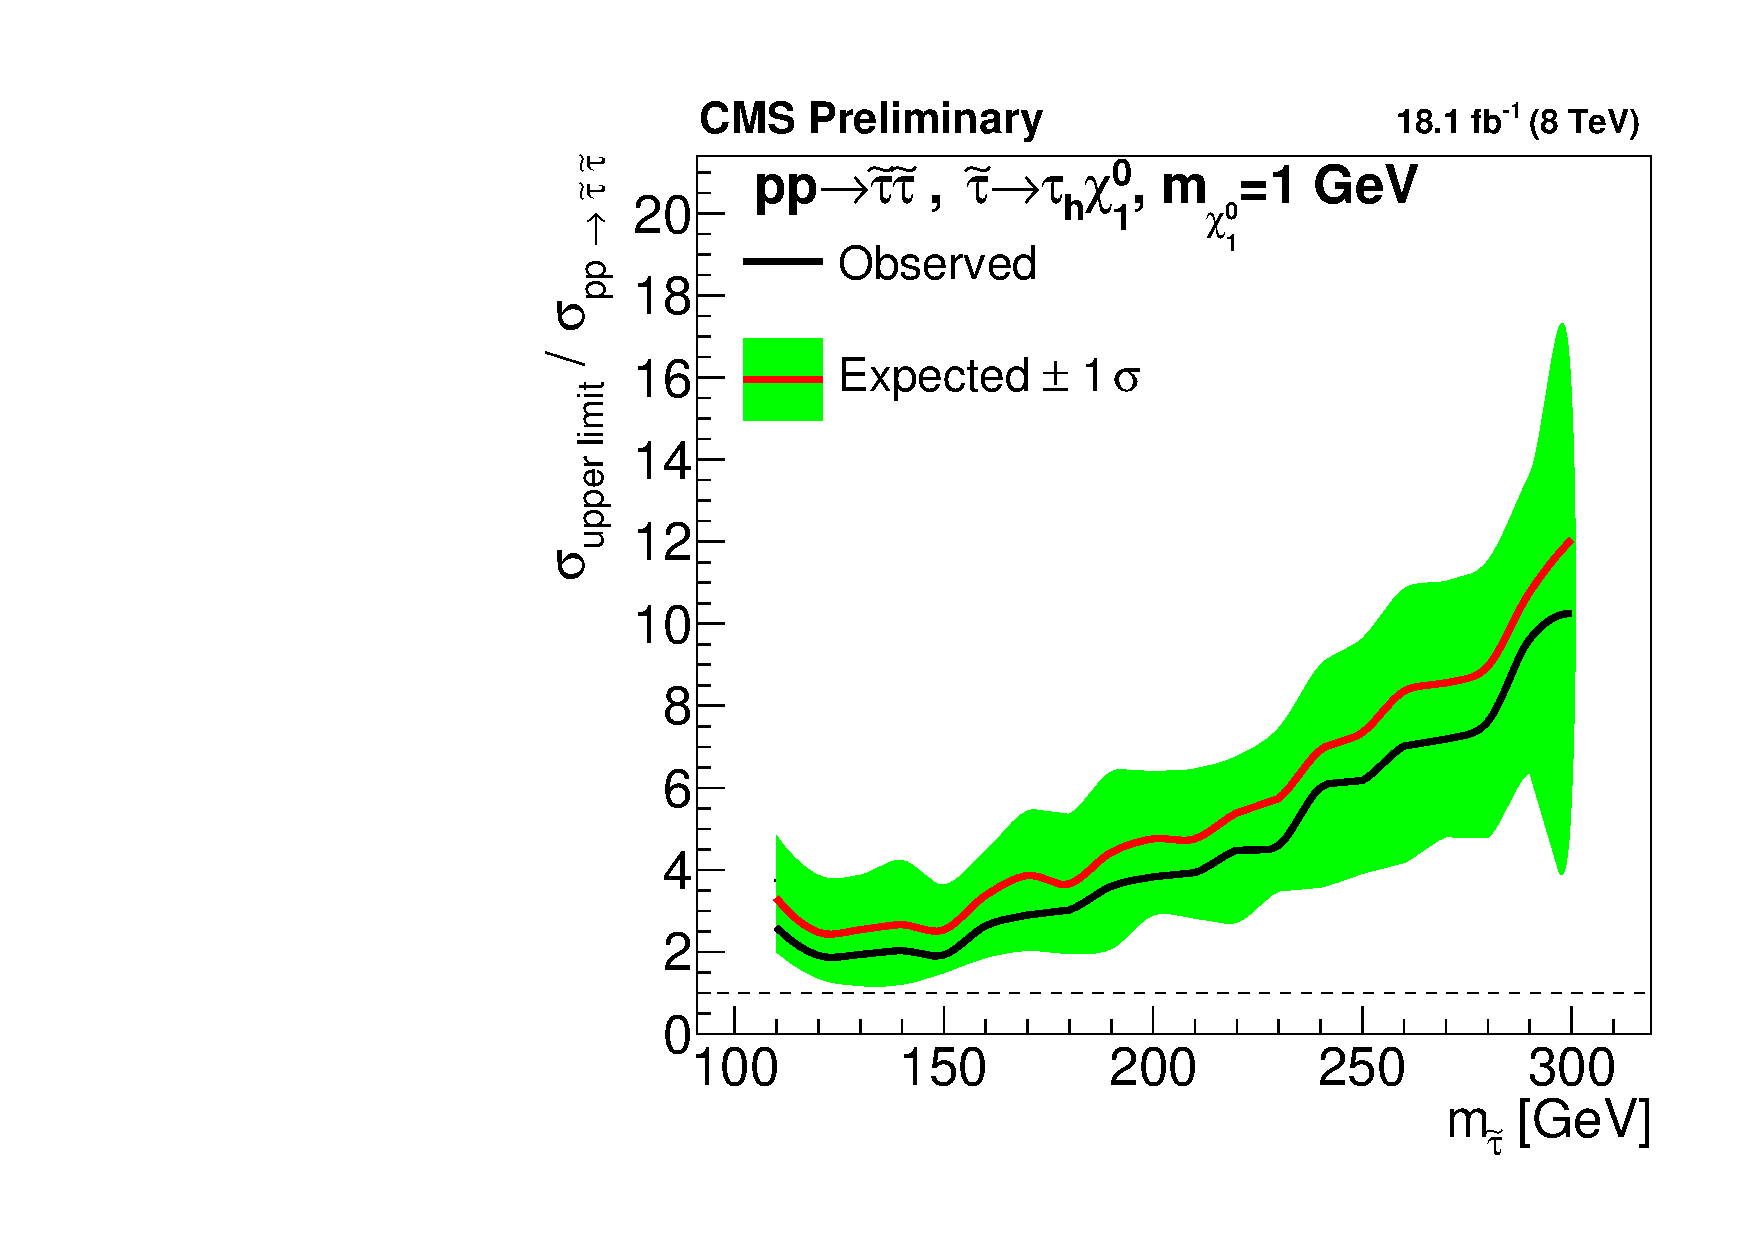
\includegraphics[width=0.5\textwidth,keepaspectratio=true]{StatisticsFig/ExclusionSTauSTauLsp1.pdf}
\caption{The exclusion power of the \tauTau channels in $\tilde{\tau}\tilde{\tau}$ production. The mass of \PSGczDo is 1\GeV.}
\label{fig:limit_stau_stau}
\end{figure}
\end{linenomath}
obtained upper limit on the cross section and the cross section expected from SUSY (signal strength) vs. the mass of the $\tilde{\tau}$ particle, when \PSGczDo mass is 1\GeV.
The observed ratio is within one standard deviation of  the expected ratio.
The best limit, which corresponds to the lowest signal strength, is obtained for $m_{\tilde{\tau}}=110\GeV$. The observed (expected) upper limit on the cross section at this mass is 228 (328) fb which is almost three times larger than the theoretical NLO cross section.



